\begin{frame}{Theoretical Security – Probing Model}

%To theoretically evaluate the security of our design, we consider the probing model .
%\pause
For a positive integer $t$,
\begin{itemize}
	\item The $t$-probing model  \cite{C:IshSahWag03} assumes that an adversary is able to peek any $t$ intermediate values in the algorithm.
	\pause
	\item To be secure in $t$-probing model, $n \geq t+1$, and any share cannot be combined with each other.
	\pause
	\item It is complicated to prove $t$-probing security for a large composition of gadgets. We apply the concept of non-interference.
\end{itemize}

\end{frame}


\begin{frame}{Non-Interference Security}

\begin{definition}{$t$-Non-Interference ($t$-NI) Security (from \cite{CCS:BBDFGS16})}
A gadget is $t$-Non-Interference ($t$-NI) secure if every set of $t$ intermediate values can be simulated by no more than $t$ shares of each of its inputs.
\end{definition}
\medskip
\pause

\begin{definition}{$t$-Strong Non-Interference ($t$-SNI) Security (from \cite{CCS:BBDFGS16})}
A gadget is $t$-Strong-Non-Interference ($t$-SNI) secure if for every set of $t_I$ internal intermediate values and $t_O$ of its output shares with $t_I + t_O \leq t$, they can be simulated by no more than $t_I$ shares of each of its inputs.
\end{definition}
\medskip

\end{frame}


\begin{frame}{Non-Interference Security}

\begin{itemize}

\item For $t = n-1$, if a gadget is $t$-NI or $t$-SNI secure, and if any $n-1$ input shares are uniformly and independently distributed, then it is $t$-probing secure.
\pause

\item All the gadgets in our paper are proven either $t$-NI or $t$-SNI secure.

\end{itemize}


\end{frame}


\begin{frame}{Non-Interference Security of Gadgets in Our Work}

\begin{table}
\centering
\begin{tabular}{l l | l l} 
\toprule
\textbf{Gadget} & \textbf{Security$\quad$} & \textbf{Gadget} & \textbf{Security$\quad$} \\
\midrule
{\sf SecAnd} & $t$-SNI & {\sf SecOr} & $t$-SNI \\
{\sf SecMult} & $t$-SNI & {\sf SecNonzero} & $t$-SNI \\
{\sf SecAdd} & $t$-NI & {\sf SecFprUrsh} & $t$-SNI \\
{\sf A2B} & $t$-SNI & {\sf SecFprNorm64} & $t$-NI\\
{\sf B2A} & $t$-SNI & {\sf SecFPR} & $t$-SNI \\
${\sf B2A_{Bit}}$ & $t$-SNI & {\sf SecFprMul} & $t$-SNI\\
{\sf RefreshMasks} & $t$-NI & {\sf SecFprAdd} & $t$-SNI\\
{\sf Refresh} & $t$-SNI \\
\bottomrule
\end{tabular}
\caption{List of gadgets in our work with $n=t+1$ shares}
\label{table:gadgets_secureity}
\end{table}
\end{frame}


\begin{frame}{Practical Security – Test Vector Leakage Assessment (TVLA)}

To test the leakage of a real device, the Test Vector Leakage Assessment (TVLA) methodology \cite{gilbert2011testing} can be applied.
\pause

A tester records two sets of traces where
\pause

\begin{itemize}
	\item Set 1: fixed input
	\pause
	\item Set 2: random input
\end{itemize}
\pause

The Welch's $t$-test is then applied on the two sets.
\pause

By convention, we consider the leakage is significant if the $t$-value exceeds $\pm 4.5$.
\pause

For long traces, we refer to \cite{ding2018towards} to alter this threshold to avoid false positives.

\end{frame}


\begin{frame}{Experiment Setup}

We implemented our design in the following setting:
\pause

\begin{itemize}
\item Plain-C code
\pause
\item Compiled by {\tt arm-none-eabi-gcc 10.3.1}
\pause
\item Using ChipWhisperer with target board STM32F415 with an ARM Cortex-M4 MCU
\pause
\item We compare the result with the reference implementation of the NIST Round-3 Submission of \textsc{Falcon} \cite{NISTPQC-R3:FALCON20}.
\end{itemize}

\end{frame}




\begin{frame}{TVLA}

The TVLA results of floating-point number multiplication (FprMul, SecFprMul).

\begin{columns}[T]
\column{.34\textwidth}
\begin{figure}
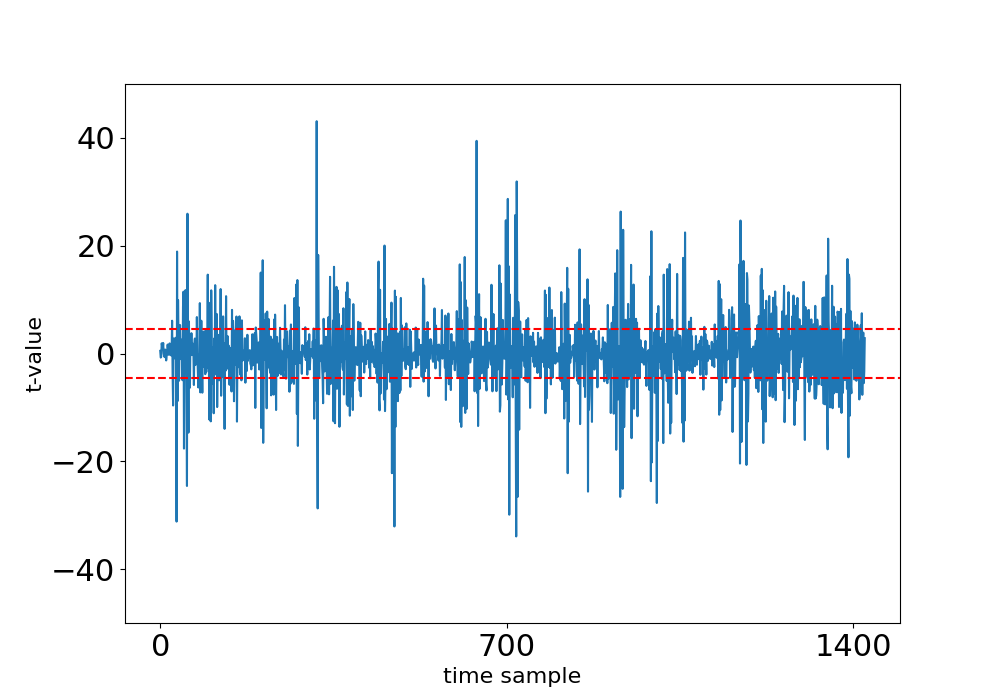
\includegraphics[width=\textwidth]{Figure/tvla-F4-CHES/fpr_mul_1k.png}
\vspace{-20pt}
\caption{1,000 traces, unmasked FprMul}
\end{figure}

\column{.34\textwidth}
\begin{figure}
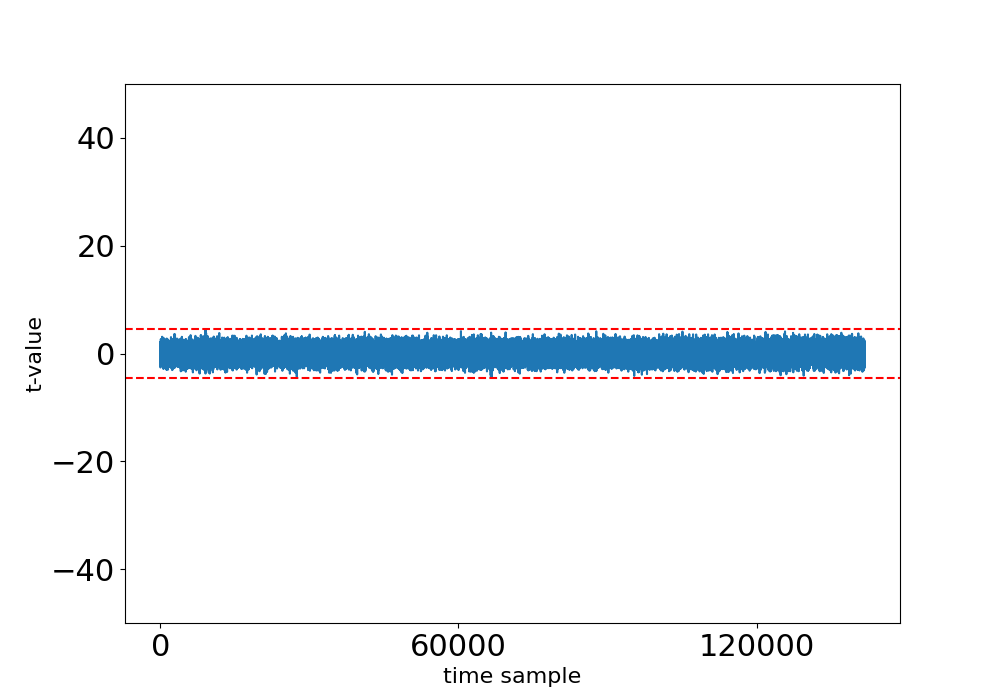
\includegraphics[width=\textwidth]{figure/tvla-F4-CHES/SecFprMul_2shares_10k.png}
\vspace{-20pt}
\caption{10,000 traces, 2-shared SecFprMul}
\end{figure}

\column{.34\textwidth}
\begin{figure}
\includegraphics[width=\textwidth]{figure/tvla-F4-CHES/SecFprMul_3shares_100k.png}
\vspace{-20pt}
\caption{100,000 traces, 3-shared SecFprMul}
\end{figure}

\end{columns}


\end{frame}



\begin{frame}{TVLA}

The TVLA results of floating-point number addition (FprAdd, SecFprAdd).

\vskip -15pt
\begin{columns}[T]
\column{.34\textwidth}
\begin{figure}
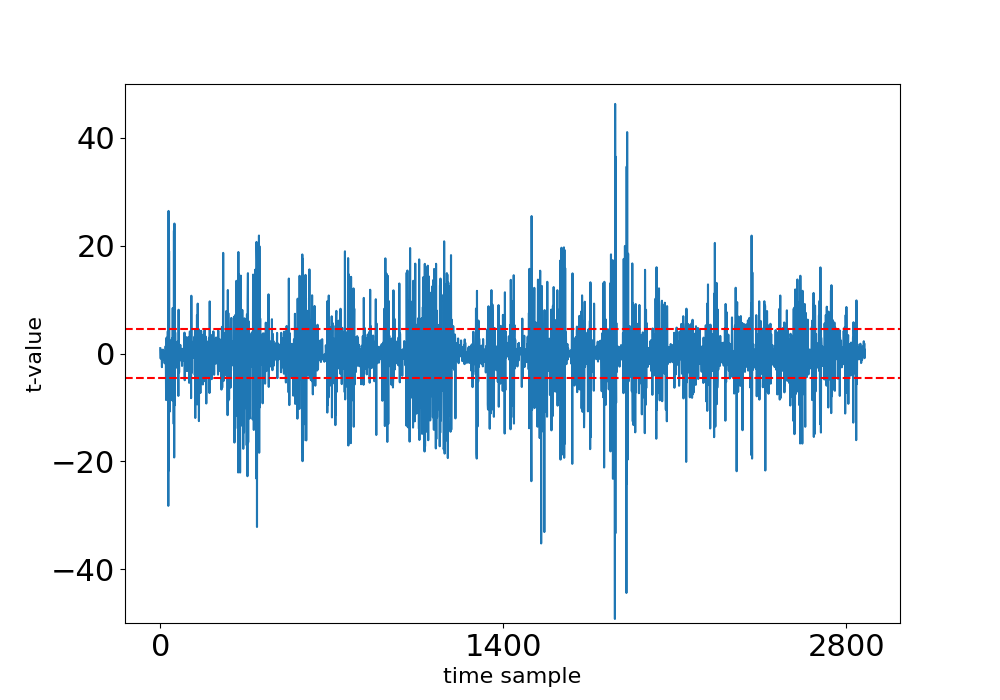
\includegraphics[width=\textwidth]{figure/tvla-F4-CHES/fpr_add_1k.png}
\vspace{-20pt}
\caption{1,000 traces, unmasked FprAdd}
\end{figure}

\column{.34\textwidth}
\begin{figure}
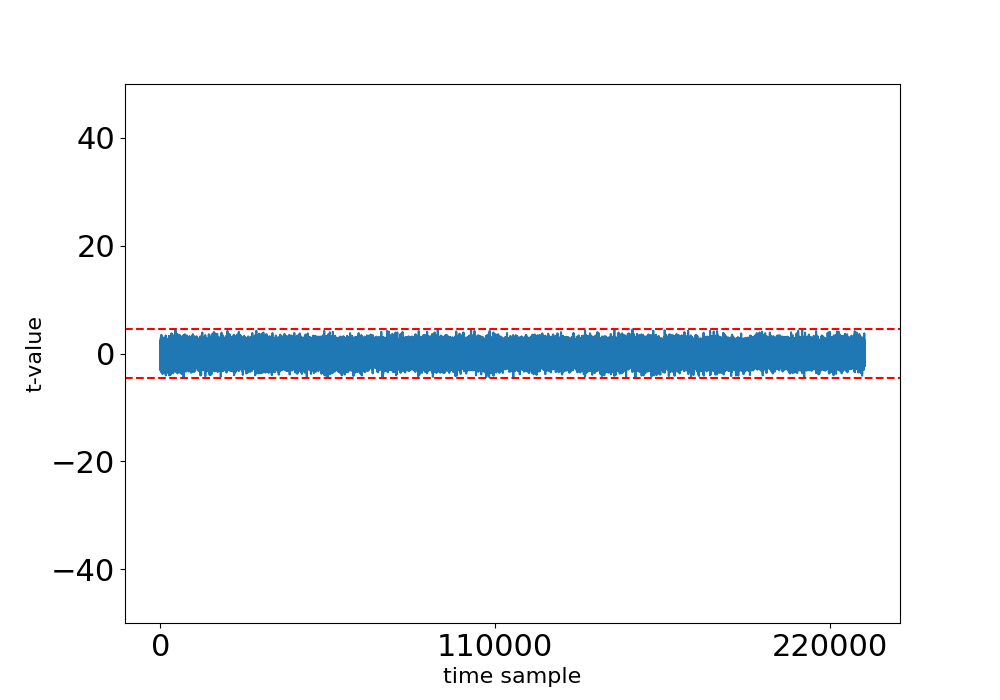
\includegraphics[width=\textwidth]{figure/tvla-F4-CHES/SecFprAdd_2shares_10k.png}
\vspace{-20pt}
\caption{10,000 traces, 2-shared SecFprAdd}
\end{figure}

\column{.34\textwidth}
\begin{figure}
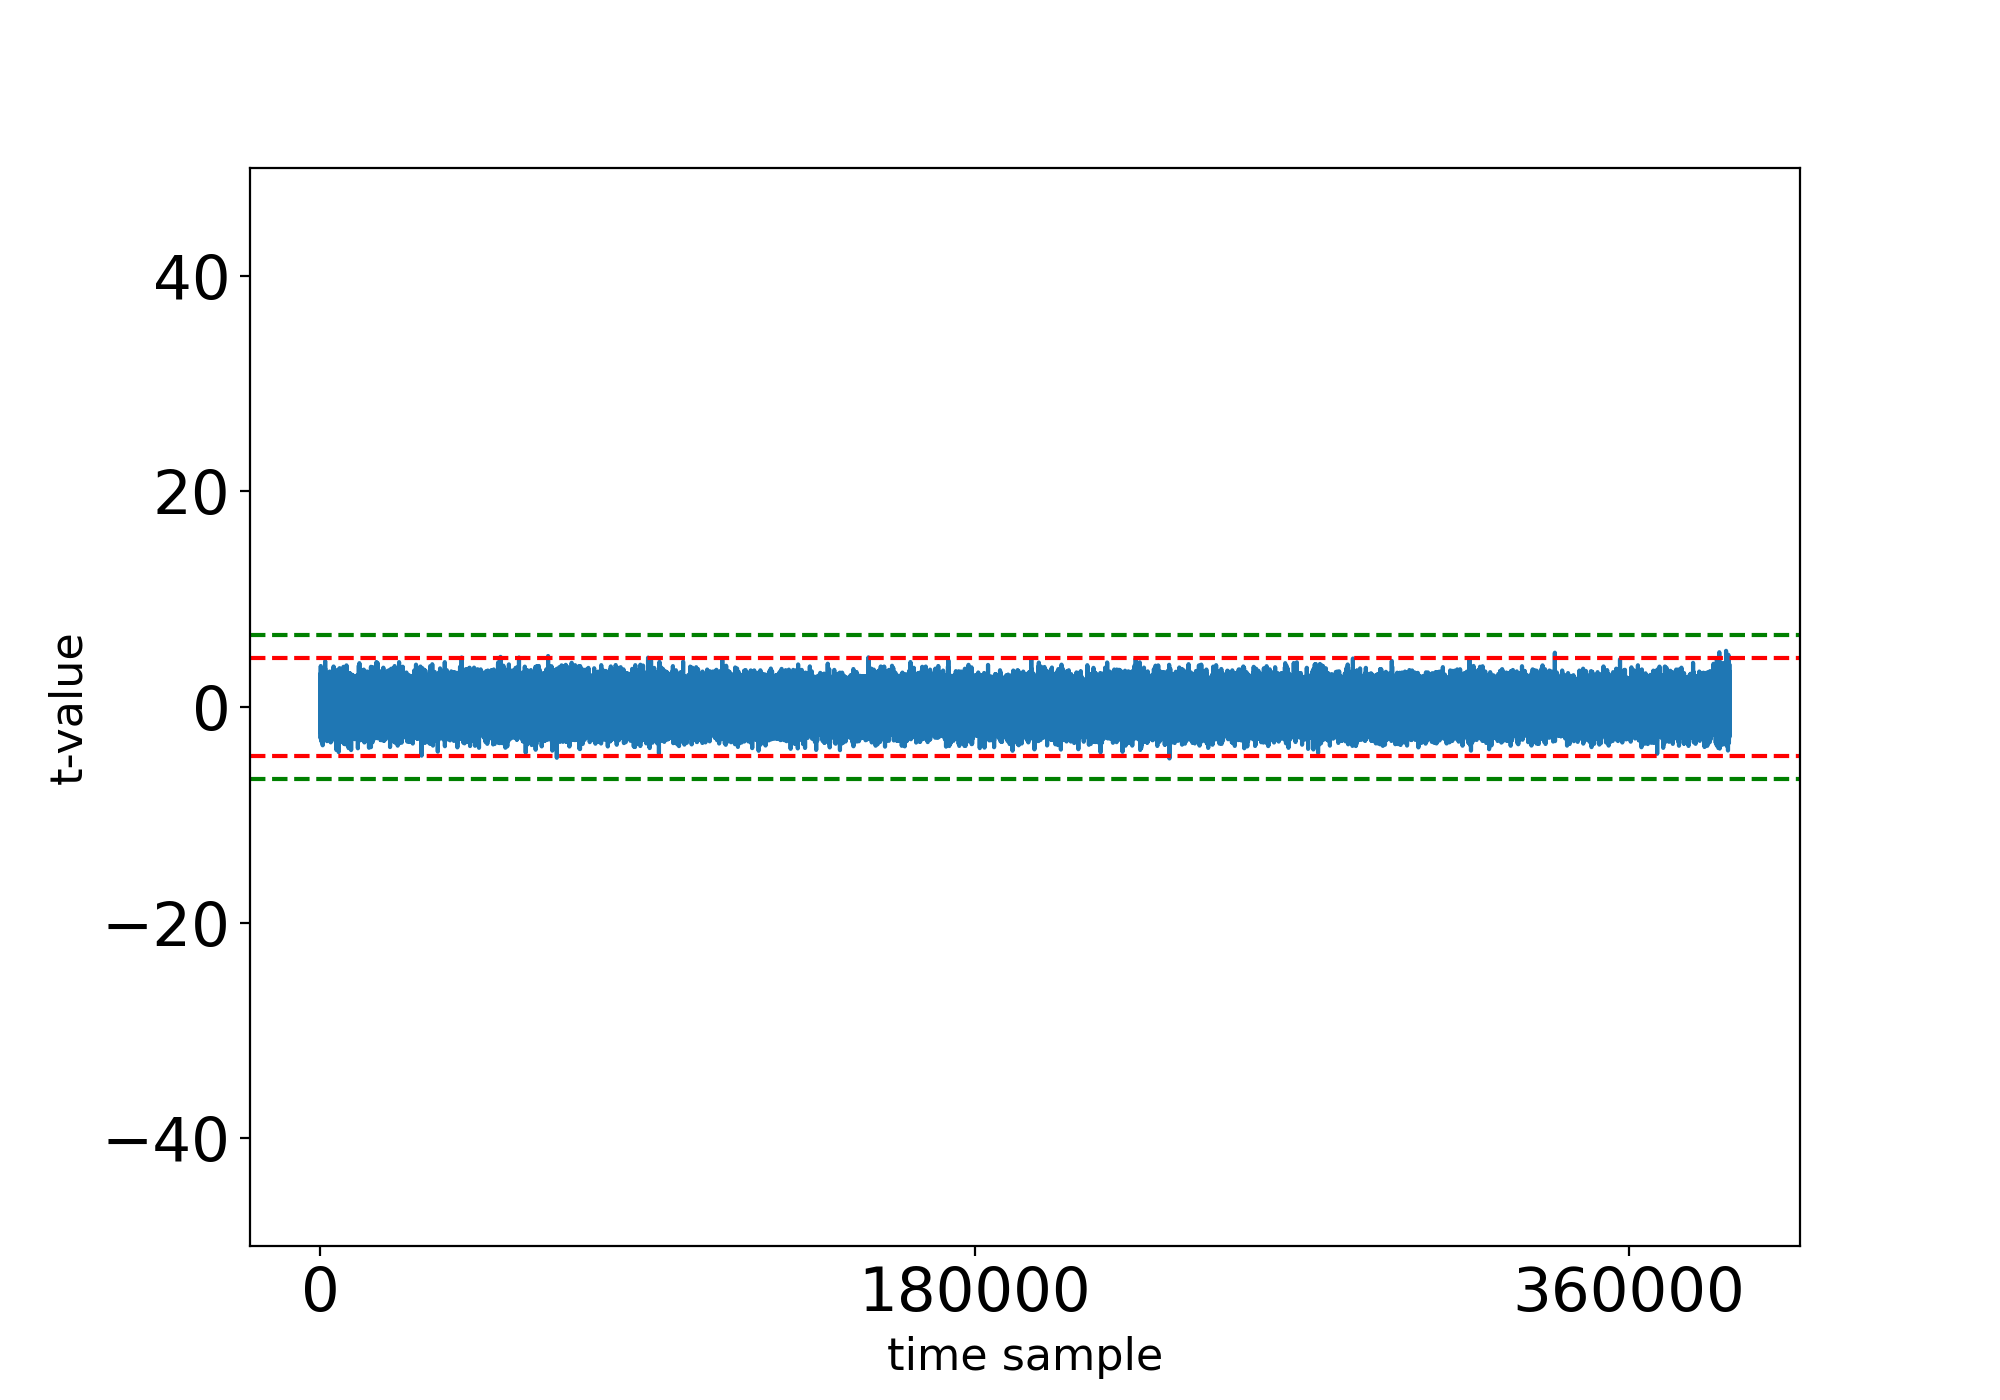
\includegraphics[width=\textwidth]{figure/tvla-F4-CHES/SecFprAdd_3shares_100k.png}
\vspace{-20pt}
\caption{100,000 traces, 3-shared SecFprAdd}
\end{figure}

\end{columns}


\end{frame}


%
%\begin{frame}{TVLA}
%
%The 3-shared version show no obvious leakage in even 100,000 traces. We adapt the thresholds (green) \cite{ding2018towards} to $\pm 6.603$ for {\sf SecFprMul} and $\pm 6.646$ for {\sf SecFprAdd}.
%
%\vskip -15pt
%\begin{columns}[T]
%\column{.5\textwidth}
%\begin{figure}
%\includegraphics[width=\textwidth]{figure/tvla/SecFprMul_3shares_100k.png}
%\vspace{-20pt}
%\caption{100,000 traces, 3-shared SecFprMul}
%\end{figure}



%\end{frame}